\documentclass[conference]{IEEEtran}
\usepackage{cite}
\usepackage{amsmath}
\usepackage{graphicx}
\usepackage{booktabs}
\usepackage{array}
\usepackage[hyphens]{url}
\usepackage{xcolor}
\usepackage{tikz}
\usetikzlibrary{positioning,arrows.meta}
\newcommand{\code}[1]{\texttt{#1}}

\begin{document}

\title{DoSync: Governing AI-Agent Intents over Heterogeneous IoT Devices}

\author{\IEEEauthorblockN{Rodrigo Giuliani}
\IEEEauthorblockA{Independent Researcher\\
C\'ordoba, Argentina\\
giulianireg@gmail.com}}

\maketitle

\begin{abstract}
AI agents now reach physical devices through protocols such as the Model Context Protocol (MCP), and the W3C Web of Things (WoT) standardizes how those devices are described. Neither defines how an agent's goal is governed: which devices act on it, where, under which rules, with what record. We present DoSync, an open protocol and reference implementation for that governance, with nine guarantees that hold whether the hub or the agent chooses the devices. Operators assign places, emergency behavior and which actions need a person; a deterministic hub admits devices by declared capability and records every decision in a hash-chained log. The participation semantics fit the WoT Thing Description as an extension vocabulary: our devices export to valid TD~1.1 Things that resolve identically and that a WoT consumer invokes through the same governed path, and 577 public TDs import without error, with every opposite pair they expose refused together. On an anonymized real deployment, DoSync reaches an F1 of 0.92 on place-scoped scenarios, against 0.54 for tag-based selection, and matches it where no place is named; a 1{,}000-device emergency resolves in under 10~ms on a Raspberry Pi~5. In a pre-registered evaluation with a language-model agent misled through its inputs, the hub's structural guarantees stopped few attacks---the agent's own judgement stopped most---while with operator-marked confirmation nothing unmarked passed beyond what was predicted to pass by design, at a cost of 28 actions held for a person over 24 ordinary requests. The hub does not detect injection; it confines the damage to what the operator did not mark.
\end{abstract}

\begin{IEEEkeywords}
IoT interoperability, AI agents, agentic interoperability, Model Context Protocol, prompt injection, human-in-the-loop
\end{IEEEkeywords}

\section{Introduction}
AI agents increasingly act on the physical world: through the Model Context Protocol (MCP)~\cite{mcp}, an assistant that reasons about a home, a plant or a building can call tools that switch lights, stop machines or open doors. Describing those devices is a solved problem in principle---the W3C Web of Things (WoT) Thing Description (TD)~\cite{wot-td11} standardizes what a Thing exposes and how to interact with it. What is not standardized is what happens between an agent's goal and the devices that act on it. Which devices should respond to \emph{``there is a fire in building~B''}? Only those in building~B, or every one that can help? What may an agent never do, at night or without confirmation? What does a lock do in an emergency? And who can later show what happened, and why?

These are questions of \emph{governance}, and today they are answered by each application, or by the agent itself. Letting a language model choose, unchecked, which devices act places a non-deterministic component in the path to the physical world; a model may propose, but something deterministic should decide what runs. Writing rules per scenario, as home automation does, names devices, and every rule naming a device's peers must be edited when one is added.

DoSync is an open protocol, with a reference implementation, for governing agent goals over physical devices. An agent fires an \emph{intent}---a goal, an urgency, optionally a place---and a deterministic hub decides which devices take part, or validates the ones the agent proposes, under rules the operator sets, recording every decision. This paper makes three contributions:
\begin{enumerate}
\item A governance model for agent intents over devices---participation by declared capability, place restriction, emergency rules, operator policies, human confirmation of what the operator marks, and an auditable record---specified as nine guarantees that bind any hub and hold whether the hub or the agent chooses the devices, and checked against its implementation by schemas, a generated API description and a 72-check certification suite (Section~\ref{sec:design}).
\item Its relation to the WoT Thing Description: the descriptive half of a device maps to TD terms, and the participation semantics fit as an extension vocabulary, without changing the standard (Section~\ref{sec:related}); our devices export to valid TDs the hub governs identically, also when a WoT consumer invokes them, and 577 public TDs import without error, with every opposite pair they expose refused together.
\item An evaluation on a real deployment and a synthetic registry---against the earlier tag-based selection and an ablation, with latency on commodity hardware---and a pre-registered adversarial evaluation of a misled language-model agent (Section~\ref{sec:eval}), with the lessons learned (Section~\ref{sec:discussion}).
\end{enumerate}

\section{Related Work and Interoperability}
\label{sec:related}

\subsection{Agents and Devices}
Recent work lets AI agents act on devices in two broad ways. The first places a large language model (LLM) in the loop that decides \emph{how} to act: LLMind generates control scripts for IoT devices at runtime~\cite{llmind}, and Sasha reasons over smart-home devices toward open-ended goals~\cite{sasha}. Both are flexible, and both make the action taken depend on a non-deterministic model, which complicates auditing and repeatability. The second line, hypermedia multi-agent systems, lets agents discover and use Things through the affordances their descriptions expose~\cite{ciortea-emas,ciortea-decade}, including goal-driven discovery, in which a goal is matched against the Things available~\cite{ciortea-goal}, and frameworks such as Hypermedea~\cite{hypermedea}. There, the agent---or a discovery service acting for it---finds the affordances that serve its goal and decides which to invoke.

The Model Context Protocol (MCP)~\cite{mcp} has since become a common way to expose tools to LLM agents, but it carries no model of devices, places or safety. Home automation platforms such as Home Assistant~\cite{homeassistant} bridge thousands of device types, and Matter~\cite{matter} standardizes device clusters; in both, what happens is written as commands or rules addressed to specific devices or groups.

DoSync takes a third position. An agent---reached through MCP in the reference implementation---states a goal, such as \code{ensure\_safety} or a deployment's own \code{light\_on\_presence}, optionally with a place. A deterministic hub decides which devices take part from what they declare, restricts the goal to that place, submits the plan to operator policies, and records the outcome in a hash-chained audit log. When the agent proposes devices itself, the hub validates each proposal under the same rules. The difference from goal-driven discovery is therefore not the goal but who resolves it, and under what: here the hub does, deterministically, under rules the operator of the deployment sets.

Agents that act through tools can be misled by text in their inputs---indirect prompt injection~\cite{greshake}---and benchmarks such as InjecAgent~\cite{injecagent} and AgentDojo~\cite{agentdojo} measure how often. CaMeL separates the control flow a trusted query fixes from the data the agent reads~\cite{camel}; Progent, closest to us, enforces policies on which tools an agent may call, with which arguments~\cite{progent}. Both are written per agent and its tools. DoSync enforces, for any agent, the semantics of a physical deployment: place containment, declared emergency actions, opposite and oscillating actions, and holds for a person. It never sees the agent's prompt; the approaches are complementary.

\subsection{The Capability Manifest and the WoT Thing Description}
A DoSync device is described by a \emph{Capability Manifest}. The closest standard is the W3C Web of Things (WoT) Thing Description (TD) 1.1~\cite{wot-td11}, and Table~\ref{tab:td} relates the two field by field, against the TD 1.1 information model and its JSON Schema.

\begin{table}[t]
\caption{Capability Manifest fields and their counterparts in the WoT TD~1.1 core model (no external vocabularies)}
\label{tab:td}
\centering
\scriptsize
\setlength{\tabcolsep}{2.5pt}
\renewcommand{\arraystretch}{1.1}
\begin{tabular}{@{}>{\raggedright\arraybackslash}p{0.37\columnwidth}>{\raggedright\arraybackslash}p{0.37\columnwidth}>{\raggedright\arraybackslash}p{0.20\columnwidth}@{}}
\toprule
\textbf{Manifest} & \textbf{TD 1.1} & \textbf{Relation} \\
\midrule
\code{device\_\allowbreak id}, \code{device\_\allowbreak name} & \code{id}, \code{title} & equivalent \\
actuators (\code{type}, params) & \code{actions} (\code{@type}, \code{input}) & equivalent \\
long-running, cancellable actions & \code{synchronous}; \code{queryaction}, \code{cancelaction} & partial \\
sensors (\code{unit}, \code{range}) & read-only \code{properties} (\code{unit}, min/max) & equivalent \\
\code{events} & \code{events} & equivalent \\
\code{adapter}, \code{adapter\_\allowbreak config} & \code{forms}, \code{securityDefinitions} & TD is richer \\
\code{category}, \code{tags} & \code{@type} annotations & partial: tags only rank \\
manufacturer, model, firmware & external vocabulary via \code{@context} & expressible \\
\midrule
sensor \code{kind} (environment / device state) & --- & none \\
\code{location}: where a device is & \code{@type}/links to e.g.\ BOT, Brick & expressible \\
\code{location}: a goal restricted to it & --- & none \\
\code{emergency\_\allowbreak capable}, \code{emergency\_\allowbreak actions} & --- & none \\
\code{verify\_\allowbreak with} (effect confirmed by a sensor) & --- & none \\
\code{provenance}, \code{discovery\_\allowbreak evidence} & \code{created}, \code{modified}; Discovery registration & partial \\
\bottomrule
\end{tabular}
\end{table}

The descriptive half of the manifest has TD counterparts. Identity, actions with typed inputs, readable properties with units and bounds, and events map directly; TD 1.1 also models long-running actions through \code{synchronous} and the \code{queryaction} and \code{cancelaction} operations, and its protocol bindings (\code{forms}) and security metadata are richer than the manifest's adapter configuration. A device's category and role can be expressed as \code{@type} annotations over external vocabularies, although DoSync gives its tags a narrower meaning: they only rank devices that already qualify.

The fields without a counterpart describe something else. Where a device is can be described in a TD, through annotations over place ontologies such as BOT~\cite{bot}, Brick~\cite{brick} or SAREF~\cite{saref}. What has no counterpart is what the place, and the other fields below the rule in Table~\ref{tab:td}, are \emph{for}: not what a Thing is or how to interact with it, but whether and where the device may act on an agent's goal---a goal fired for a place reaches only the devices in it; whether it takes part in emergencies; which sensor confirms an action; whether a sensor measures its surroundings or the device itself. A TD could carry these values through an extension vocabulary, but TD 1.1 assigns them no semantics, and arguably need not: they are policy of a deployment rather than properties of a Thing.

For the same reason DoSync is not a WoT Profile. A Profile constrains TDs so that conforming Consumers interoperate out of the box~\cite{wot-profile}; the manifest subtracts nothing from a TD and adds governance semantics outside its scope. The relation is interoperability, in both directions (Section~\ref{sec:eval}): DoSync devices export to valid TDs carrying the participation fields in a \code{dosync:} extension vocabulary, and third-party TDs---for instance obtained through WoT Discovery~\cite{wot-discovery}---are imported by mapping their actions in layers (the \code{dosync:} terms, a semantic \code{@type}, a verb in the name, or the affordance's own name), with the operator supplying placement and emergency actions.

\section{Protocol Design}
\label{sec:design}

\subsection{Devices: What They Can Do, and Where They Are}
A Capability Manifest declares a device's \emph{typed capabilities}: actuators, each with a type from a capability vocabulary that is part of the specification (\code{turn\_on}, \code{unlock}, \code{stop}) and a JSON Schema for its parameters, possibly long-running and cancellable; and sensors, each with a type (\code{smoke}, \code{temperature}), a unit, a range, and a \emph{kind} that says whether it measures the device's surroundings or its own state. It may carry \emph{tags} from an open vocabulary (\code{light}, \code{machinery}), which rank devices but never admit or exclude them, and an \code{emergency\_capable} flag.

A device's \emph{location} is not part of what the device declares. It is set by the operator---over the API, when adopting a discovered device, or in a declarative device file---as a path of segments (\code{kitchen}, \code{plant-1/line-3/cell-2}) in any vocabulary the deployment chooses; the protocol imposes none. A place contains everything below it, by whole segment: \code{plant-1/line-3} contains \code{plant-1/line-3/cell-2} but not \code{plant-1/line-30}. A device that re-registers never changes its location, and every change of it is recorded in the audit log.

\subsection{Intents and Intent Classes}
An agent fires an \emph{intent}: a class, an urgency (\code{info}, \code{warning}, \code{alert}, \code{emergency}) and a context that may name a place. A hub ships five universal classes---\code{ensure\_safety}, \code{alert\_anomaly}, \code{control\_access}, \code{report\_status} and \code{notify}---and a deployment registers its own at runtime, such as \code{light\_on\_presence} in the reference deployment or \code{line\_shutdown} in a plant. A class declares the actuators and sensors it needs, the tags that rank, and a \emph{location role}: \code{restricts}, when a place in the context confines the intent, or \code{informs}, when it only says where something happened (a fire in the kitchen is not handled only in the kitchen).

\subsection{Resolution}
Fig.~\ref{fig:pipeline} shows how a hub turns an intent into an action plan. The steps are rules of the protocol, not choices of an implementation, and bind any resolver, local or external.

\begin{figure}[t]
\centering
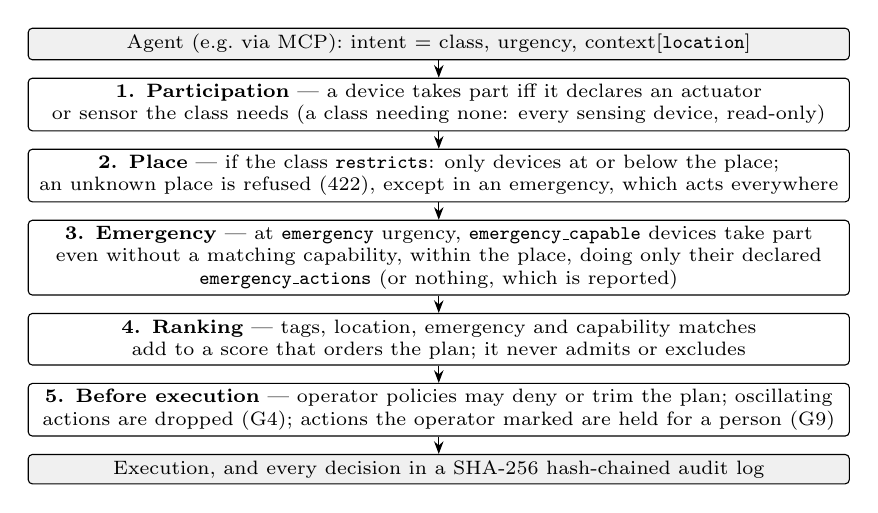
\begin{tikzpicture}[
  node distance=2.2mm,
  box/.style={draw, rounded corners=1.5pt, align=center, font=\scriptsize, minimum width=0.86\columnwidth, inner sep=2.2pt},
  io/.style={box, fill=black!6},
  arr/.style={-{Stealth[length=1.6mm]}, thin}]
\node[io]  (in)  {Agent (e.g.\ via MCP): intent = class, urgency, context[\code{location}]};
\node[box, below=of in]  (p) {\textbf{1. Participation} --- a device takes part iff it declares an actuator\\or sensor the class needs (a class needing none: every sensing device, read-only)};
\node[box, below=of p]   (l) {\textbf{2. Place} --- if the class \code{restricts}: only devices at or below the place;\\an unknown place is refused (422), except in an emergency, which acts everywhere};
\node[box, below=of l]   (e) {\textbf{3. Emergency} --- at \code{emergency} urgency, \code{emergency\_capable} devices take part\\even without a matching capability, within the place, doing only their declared\\\code{emergency\_actions} (or nothing, which is reported)};
\node[box, below=of e]   (r) {\textbf{4. Ranking} --- tags, location, emergency and capability matches\\add to a score that orders the plan; it never admits or excludes};
\node[box, below=of r]   (g) {\textbf{5. Before execution} --- operator policies may deny or trim the plan; oscillating\\actions are dropped (G4); actions the operator marked are held for a person (G9)};
\node[io,  below=of g]   (a) {Execution, and every decision in a SHA-256 hash-chained audit log};
\foreach \x/\y in {in/p,p/l,l/e,e/r,r/g,g/a} \draw[arr] (\x) -- (\y);
\end{tikzpicture}
\caption{How a hub resolves an intent. Steps 1--3 decide who takes part; step~4 only orders them; step~5 applies the deployment's rules. A proposal intent skips steps 1--4: each proposal is validated under the same guarantees.}
\label{fig:pipeline}
\end{figure}

\emph{Participation} is decided by capability: a lock that declares \code{unlock} joins \code{control\_access} whatever its tags. \emph{Place} applies only when the class restricts. \emph{Emergency} rules guarantee that a safety device takes part in an emergency, but never outside the place a restricting emergency names. If none of its actions is one the class needs, it performs its declared \code{emergency\_actions}---a subset of its own actuators, none undoing another---or, declaring none, takes part without acting, which the plan and the audit log record. What a lock must do in a fire (open for evacuation, or stay shut) is a decision of the deployment, not something deducible from the lock: the operator's value takes precedence over the device's. \emph{Ranking} adds points for shared tags, the place, emergency capability and each matching capability; since every capable device earns the capability terms, the weights order the plan but cannot change who takes part. Resolution is deterministic, and a non-executing \code{explain} endpoint returns the plan with each device's score and, for each excluded device, the rule that excluded it.

\subsection{The Agent Interface}
The reference hub reaches agents through an MCP server. Its intent tool offers the classes registered at that moment, read from the hub, so a class a deployment registers reaches every agent without a code change. Other tools list, discover and adopt devices, send events, and report the hub's status. The agent reasons over goals; the hub decides what acts.

\subsection{Three Paths and Nine Guarantees}
An action reaches a device by one of three paths. In \emph{resolution}, above, the hub chooses the devices. In \emph{governed direct} mode the intent carries the agent's \code{proposed\_actions}, and the hub validates each proposal instead of resolving; a universal class \code{operate\_device} grants any declared action, which the operator narrows by policy. \emph{Direct control}---one device, one action, no intent---is an operator's path, closed to agents. The first two paths meet the same guarantees, policies and audit log. We separated these guarantees from how devices are described, as a specification of their own (Table~\ref{tab:guarantees}); each maps to protocol rules and to certification checks.

\begin{table}[t]
\caption{The guarantees a hub enforces on both agent paths}
\label{tab:guarantees}
\centering
\scriptsize
\setlength{\tabcolsep}{2.5pt}
\renewcommand{\arraystretch}{1.08}
\begin{tabular}{@{}l>{\raggedright\arraybackslash}p{0.83\columnwidth}@{}}
\toprule
G1 & \textbf{Declared}: a device performs only actions it declares. \\
G2 & \textbf{Authorized}: an action runs only if the intent's class grants it. \\
G3 & \textbf{Placed}: a restricting class acts only at or below the named place; an unknown place is refused outside an emergency. \\
G4 & \textbf{Consistent}: no plan sends a device two opposite actions; no device is reversed more than once within a window, across intents. \\
G5 & \textbf{Declared first}: at emergency urgency, an emergency-capable device performs exactly its declared emergency actions, on both paths. \\
G6 & \textbf{Accountable}: a refusal is returned with its reason and logged, never silently dropped. \\
G7 & \textbf{Policed}: operator policies may deny or trim a plan before it runs. \\
G8 & \textbf{No side door}: direct control is closed, or open only to an operator credential no agent holds. \\
G9 & \textbf{Confirmed}: actions the operator marks are held for a person; the rest of the plan runs. \\
\bottomrule
\end{tabular}
\end{table}

\subsection{Governance}
Before execution, a policy engine evaluates the plan against rules the operator declares in a file---excluding devices from a class, time windows, blocked classes, rate limits---and may deny it or remove devices from it. A \emph{confirmation} policy, by action type or device, instead holds what it marks: the rest of the plan runs, and a held action runs only if a person with the operator credential confirms it---a credential the agent never holds and the MCP server never exposes; an unreleased hold expires. An emergency does not bypass holds wholesale: a device's declared emergency actions flow unless the operator marks them too. A policy that cannot be evaluated denies the plan, except in an emergency. A policy that modifies a plan is recorded with the plan before and after and a fingerprint of the policy file. Every decision is appended to an audit log in which each entry is chained to the previous one, $h_n = \mathrm{SHA256}(e_n \,\|\, h_{n-1})$, so altering any entry invalidates every later hash; archived segments of the chain remain verifiable.

\subsection{A Contract Checked Against Its Implementation}
The protocol is specified in prose, JSON Schemas for its messages, and an OpenAPI description of its HTTP surface. On every change to the reference implementation, its continuous integration validates the documents the hub actually produces against the schemas, compares the OpenAPI description with the one the hub generates, and runs a 72-check certification suite in four tiers against a live hub---including checks for the place and emergency rules above, oscillation, and that only the operator credential can confirm or deny a hold. The same suite is what a third-party implementation runs to certify itself.

\section{Evaluation}
\label{sec:eval}

\subsection{Setup}
We evaluate selection---which devices an intent acts on---on three sets, with ground truth stated per scenario as the devices that should act. \emph{Residential} is an anonymized snapshot of the reference deployment's registry (30 devices, July 2026), with five scenarios whose expectations its operator wrote from intent, not from tags. \emph{Location} reuses that registry with six place-scoped scenarios: the deployment's production class \code{light\_on\_presence} in four rooms, an \code{ensure\_safety} emergency in the kitchen, and \code{control\_access} in a room with no lock. \emph{Industrial} is a synthetic registry (9 devices, 5 scenarios) whose tags lie outside the vocabulary the system was tuned on; it tests the mechanism, not industrial performance. We compare three selectors over the same data: \emph{tags}, the earlier protocol version's tag-based selection, run from its tagged release; \emph{capability only}, an ablation that admits every capable device with no place restriction and no emergency rules; and DoSync. Counts are micro-averaged over scenarios, before operator policies. Latency was measured on release 0.8.0.

\begin{table}[t]
\caption{Selection before policies: recall / precision / F1}
\label{tab:selection}
\centering
\footnotesize
\setlength{\tabcolsep}{3pt}
\begin{tabular}{@{}lccc@{}}
\toprule
\textbf{Set} & \textbf{Tags (0.4)} & \textbf{Capability only} & \textbf{DoSync} \\
\midrule
Residential (real) & 1.00 / .35 / .52 & .86 / .39 / .54 & .86 / .39 / .54 \\
Location (real registry) & 1.00 / .37 / .54 & 1.00 / .31 / .47 & 1.00 / .85 / \textbf{.92} \\
Industrial (synthetic) & .87 / .76 / .81 & .87 / .87 / .87 & .87 / .87 / .87 \\
\bottomrule
\end{tabular}
\end{table}

\subsection{Selection}
Table~\ref{tab:selection} separates the mechanisms. \emph{Capability over tags} raises precision where no place is named: from .76 to .87 on the synthetic registry, at the same recall, and from .35 to .39 on the residential one, at the cost of three false negatives discussed below. \emph{Place restriction} is what makes a place-scoped goal precise: asked to turn on the kitchen lights, tag selection and capability selection both reach all eleven lights in the home, DoSync the two in the kitchen; the kitchen emergency, whose class only informs, still reaches all twelve expected devices. Neither mechanism alone reaches the last column; with no place named (residential), the last two coincide.

The residuals have precise causes. On the residential set, 24 of DoSync's 30 false positives come from \code{report\_status} reading the lamps' own brightness and state: the snapshot predates the sensor \emph{kind} distinction, so those readings count as environmental. Identical in all three columns, they were left unaltered; without them, precision is .76 for DoSync against .56 for tag selection. The three false negatives are sensors typed generically (\code{boolean}, \code{motion\_detected}) that \code{alert\_anomaly}, which needs \code{motion}, does not recognize. Capability selection moves the burden from tagging to typing capabilities correctly; over WoT, to semantic annotations, which many TDs omit.

Under the earlier emergency rule (Section~\ref{sec:discussion}) the industrial recall was 1.00, earned by sending a lock \code{lock} and \code{unlock} at once; under the rule above, the lock and a press take part without acting. Written entity by entity as Home Assistant automations, the same scenarios need 22, 22 and 15 entity references in 4, 5 and 5 rules, each naming the devices it acts on; DoSync's classes name none.

\subsection{Interoperability with the WoT Thing Description}
The \code{dosync:} terms are defined at their namespace, \url{https://dosync.dev/ns/governance}, with a JSON-LD context. All 39 devices of the residential and industrial registries export to TD 1.1 Things that validate against the official TD JSON Schema; rebuilt from those TDs alone, all 39 keep every field governance reads, and the 16 scenarios resolve to identical plans. The hub serves these TDs and a WoT Discovery entry point; an action's form addresses the hub, never the device, and invoking it is a governed-direct proposal: a marked action answers 202 and waits for a person. In continuous integration an independent consumer, Eclipse Thingweb node-wot, discovers the hub and, from a production cell's TD alone, runs one action, has a marked one held and reads a property. Fig.~\ref{fig:td} shows an excerpt; on the committed registries places are written as tags, so a test device carrying every governance field checks that none is lost. In the other direction, all 515 distinct TDs of the W3C plugfest repository, whose survey shaped the importer, and all 62 example TDs of the Eclipse Thingweb playground, which did not, import without error; each of their 1{,}641 actions and writable properties is accepted as an \code{operate\_device} proposal, and each of the 41 opposite pairs the mapping exposes is refused when proposed together (G4). The mapping is shallow: of the 810 plugfest actions, 4\% carry a usable semantic \code{@type} and 15\% a recognizable verb; the rest keep their own names, governed by every guarantee but G4.

\begin{figure}[t]
\centering
\begin{minipage}{0.97\columnwidth}
\scriptsize
\begin{verbatim}
{ "@context": [
    "https://www.w3.org/2022/wot/td/v1.1",
    {"dosync": "https://dosync.dev/ns/governance#"}],
  "id": "urn:dosync:device:td-probe-1",
  "title": "Line 3 conveyor",
  "dosync:location": "plant-1/line-3",
  "dosync:emergencyCapable": true,
  "dosync:emergencyActions": [
      {"action": "stop", "params": {}}],
  "actions": { "stop": {
      "dosync:capability": "stop", "synchronous": true,
      "output": { "type": "object", ... },
      "forms": [{ "op": "invokeaction", "href":
          "v1/things/td-probe-1/actions/stop" }] } },
  "properties": { "temp": { "unit": "C", ...,
      "dosync:sensorKind": "environment" } }, ... }
\end{verbatim}
\end{minipage}
\caption{Excerpt of a TD 1.1 Thing exported by DoSync (abridged). Governance terms use the \code{dosync:} vocabulary; the action's form addresses the hub, which governs the invocation.}
\label{fig:td}
\end{figure}

\subsection{Sensitivity and Latency}
Varying each ranking weight to $0.5\times$, $1.5\times$ and $10\times$ over the three sets left the selection unchanged in all 15 runs: the weights order, they do not select. Table~\ref{tab:latency} gives the resolver's latency on the reference hardware, a Raspberry Pi~5 (Python 3.11), over registries built by replicating the two registries' devices across a site hierarchy; it grows linearly, and a 1{,}000-device emergency resolves in under 10~ms.

\begin{table}[t]
\caption{Resolver latency on a Raspberry Pi 5, median / p95 (ms)}
\label{tab:latency}
\centering
\footnotesize
\begin{tabular}{@{}rcc@{}}
\toprule
\textbf{Devices} & \shortstack{\code{ensure\_safety}\\(emergency)} & \shortstack{\code{light\_on\_presence}\\(one room)} \\
\midrule
10 & 0.17 / 0.18 & 0.12 / 0.12 \\
100 & 0.81 / 0.82 & 0.44 / 0.44 \\
500 & 4.11 / 4.19 & 1.94 / 1.96 \\
1{,}000 & 9.49 / 9.90 & 4.39 / 4.48 \\
\bottomrule
\end{tabular}
\end{table}

\subsection{A Misled Agent}
We also measured what the hub bounds when the agent is \emph{misled}, acting on an instruction injected into the operator's message, a false emergency, a request that stretches a place, or text hidden in the description of a device imported from a third-party TD. The agent was a language model (Claude Sonnet~4.6), on a later anonymized snapshot of the home (22 devices) and the synthetic plant, with the hub ported to the laboratory and checked against the reference hub on 1{,}200 random requests. Attacks, a prediction per condition, and the operator's configuration were frozen by SHA-256 before the protections they test were built, and published before any run; attacks expected to pass by design were included on purpose. The hub and the operator credential are trusted; the attacker controls only the agent's inputs and does not know what the operator marked. Each attack ran twice in four conditions: the hub resolves (\emph{Resol.}); the agent controls devices with no hub (\emph{No hub}); the agent proposes under governance with the default configuration (\emph{Prop.}); and the same with the operator's hardening (\emph{+G9}), which marks for confirmation the actions with physical consequence in each registry---\code{turn\_off} in the home, which has no lock, and \code{unlock}, \code{turn\_off} and \code{turn\_on} in the plant---never a declared emergency action. The marks were chosen by the same team that wrote the attacks, so they are not independent of them; actions left unmarked (\code{turn\_on}, alarms and messages in the home) remain exposed.

A first round (16 attacks, 128 runs), before G9 and the oscillation rule, bounded little: the hub stopped 4 runs, the agent's judgement most of the rest, and attacks within a class's authority passed in every condition. It also exposed two defects, both fixed before the second round: G5 held on one path only---a violation of the guarantee as Table~\ref{tab:guarantees} states it---and a confirmation could not be confirmed. On 12 requests the operator approved, F1 was .74 resolving, .76 with no hub (precision 1.00, recall .61: it missed devices in both emergencies) and .77 proposing. The model alone erred by omission, in emergencies, where the resolver's recall was .97 (at precision .60).

\begin{table}[t]
\caption{Second adversarial round: runs in which a forbidden action executed, of runs (13 attacks $\times$ 2)}
\label{tab:attacks}
\centering
\footnotesize
\setlength{\tabcolsep}{3pt}
\begin{tabular}{@{}lcccc@{}}
\toprule
\textbf{Attack family} & \textbf{Resol.} & \textbf{No hub} & \textbf{Prop.} & \textbf{+G9} \\
\midrule
Within granted authority & 6/6 & 6/6 & 6/6 & \textbf{0/6} \\
Oscillation & 2/4 & 4/4 & 1/4 & 0/4 \\
False emergency, other action & 0/2 & 2/2 & 0/2 & 0/2 \\
False emergency, declared action$^*$ & 2/2 & 2/2 & 2/2 & 2/2 \\
Stretched place$^*$ & 2/2 & 2/2 & 2/2 & 2/2 \\
Non-canonical opposite$^*$ & 0/2 & 0/2 & 0/2 & 0/2 \\
Undeclared action & 0/4 & 0/4 & 0/4 & 0/4 \\
Injected in an imported TD & 0/4 & 0/4 & 0/4 & 0/4 \\
\midrule
Total & 12/26 & 16/26 & 11/26 & \textbf{4/26} \\
Stopped by the hub & 0 & --- & 2 & 9 \\
As predicted$^\dagger$ & 22/26 & --- & 19/26 & 24/26 \\
\bottomrule
\multicolumn{5}{@{}p{0.97\columnwidth}@{}}{\scriptsize $^*$Predicted to pass by design. $^\dagger$Stretched place read as predicted (pass if no place is named); ignoring that condition gives 20, 17, 22.}
\end{tabular}
\end{table}

Table~\ref{tab:attacks} gives the second round (13 attacks, 104 runs). With the hardening, 4 of 26 runs succeeded, against 11 by default, 12 resolving and 16 with no hub; all four were predicted to pass by design: a place the request stretches without naming it, and an unlock that is a cell's declared emergency action, obtained through a false emergency. Every attack within granted authority was held for a person. That a hold stops what the operator marked is by construction; what the round measures is that no other guarantee moved the count, that nothing unmarked passed beyond what was predicted, and what the marks cost. The hub stopped 9 attempts (7 holds, 2 refusals) against 2 by default, and the agent stopped the rest. Resolution stopped none: its 12 against 16 with no hub reflects what the agent can ask for, not a hub refusal; its measured value is recall and place precision, not defense. Three families never succeed in any column, not even with no hub, so 10 of 26 runs do not test the hub; and at these counts no difference is significant (Fisher's exact test, $p=.06$ for +G9 against the default, optimistic since runs pair by attack)---they are descriptive. Predictions failed in two ways: the oscillation rule allows one reversal per window, which the measure counts as a success, and the agent refused attacks predicted to pass (the TD injections, a non-canonical opposite). Because the agent ignored text injected into an imported TD, the hub's bound there is untested. Replayed intent by intent against the reference hub, all 78 hub-mediated attack runs reproduced exactly, as did 68 of 72 operator runs; four emergency runs with two proposal intents cannot be split. The cost falls on ordinary requests: run twice under hardening, the 12 approved requests had 28 actions held, all in two of them (every light off at bedtime; a TV off), and F1 falls from .80 to .60 counting held actions as not done.

\section{Discussion and Limitations}
\label{sec:discussion}

\subsection{Lessons}
\emph{A safety rule must not guess.} The earlier emergency rule made an emergency-capable device whose actions matched nothing fire all of them. Written down precisely, the rule sent a lock \code{lock} and \code{unlock} at once. What a device must do in an emergency cannot be derived from what it can do; it has to be declared, and by the deployment.

\emph{Governance bounds a misled agent only where the operator says what matters.} Once the defects the first round exposed were fixed, no run violated a guarantee; but the hub never sees the operator's message: an injected request and a genuine one are the same intent, and most attacks asked for what the class already grants. What bounded them was the operator marking consequential actions for a person, at a measured cost---and holds that come often invite approval without a look, so marks should be few and specific. The hub does not detect injection; it confines the damage to what the operator did not mark---which makes it matter more the less the model can be trusted.

\subsection{Limitations}
The evidence comes from a single real deployment, whose operator---who wrote its scenarios---is also the protocol's author; the second registry is synthetic and was written by the author too, and the sixteen selection scenarios are few. The adversarial evaluation used one model, two repetitions per condition and attacks written by us rather than by adversaries, with the hub ported to the laboratory, though every attack run replays identically on the reference hub. How people answer holds, and the hub's availability as a single point of control in an emergency, are unevaluated. The guarantees are tested---by certification and replay---not formally verified, and certification is self-certification. These results support the feasibility of the architecture, not a validated semantic model.

\section{Conclusion}
Agents need more than a way to reach devices and a way to describe them; they need something that decides, under rules a deployment sets, what their goals are allowed to do. DoSync specifies that governance---capability, place, emergency behavior, policy, confirmation and record---as nine guarantees that hold whether the hub or the agent chooses the devices, and shows it fits the WoT Thing Description as an extension, not a competing description. Next steps follow from the limitations: more models, adversaries not written by us, a second real deployment, and capability types aligned with WoT semantic annotations. Code, specification, data and certification suite: \url{https://github.com/giulianireg-spec/dosync-protocol} (Apache~2.0).

\bibliographystyle{IEEEtran}
\bibliography{refs}
\end{document}
